\usetikzlibrary{shapes,arrows,calc}

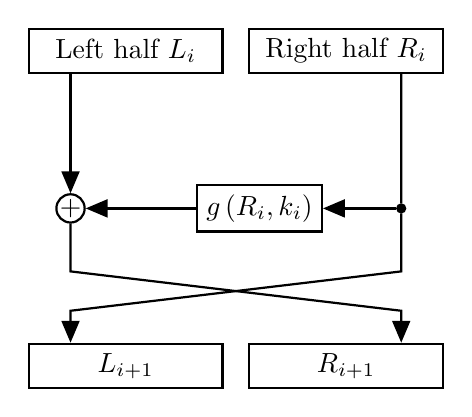
\begin{tikzpicture}
[
auto, thick, >=triangle 45,
block/.style    = {draw, thick, rectangle, minimum height = 1.6em, },
]
\node at (0,0)[block,minimum width = 7em] (left) {Left half $L_i$}; 
\node at (2.8,0)[block,minimum width = 7em] (right) {Right half $R_i$}; 

\node at (-.7,-2)[circle,draw,inner sep=0pt,minimum width=3mm] (xor) {+};
\node at (1.7,-2)[block] (f) {$g\left(R_i, k_i\right)$}; 

\node at (3.5,-2)[circle,draw,fill,inner sep=0pt,minimum width=1mm] (dot) {};

\node at (0,-4)[block,minimum width = 7em] (left2) {$L_{i+1}$}; 
\node at (2.8,-4)[block,minimum width = 7em] (right2) {$R_{i+1}$};

\draw[-] ($(right.south) + (0.7,0)$) -- ($(dot.north)$);
\draw[->] ($(dot.south)$) -- (3.5,-2.8) -- (-0.7,-3.3) -- ($(left2.north) - (0.7,0)$);
\draw[->] (dot) -- (f); 
\draw[->] (f) -- (xor);
\draw[->] ($(left.south) - (.7,0)$) -- (xor);
\draw[->] (xor) -- (-0.7,-2.8) -- (3.5,-3.3) -- ($(right2.north) + (0.7,0)$);
\end{tikzpicture} 
  